\chapter{Experiments} \label{experiments}

\section{CycleGANs with depth data}

We proposed a set of experiments in order to determine which of the GAN variants performed better for the LiDAR-like images in the CycleGAN~\cite{cyclegan} setting. Therefore all of the experiments were the same except the used loss functions for generator and discriminators. There were altogether six experiments -- original GAN~\cite{origgan}, LSGAN~\cite{lsgan} and WGAN-GP~\cite{wgan-gp} with and without self-regularization~\cite{historypool} term in the generators' loss function. We used mini-batches of size 4 (due to the memory limit of used GPUs) and trained all the networks for 80000 steps resulting in approximately 37 runs through all the training data for GTA dataset and about 32 runs for Valeo dataset. It makes no sense to use the term epoch in the setting of two different dataset with various magnitudes.

The only difference in the architecture was the use of Layer normalizations~\cite{layernorm} for the WGAN-GP instead of Batch normalizations~\cite{batchnorm} for the GAN and LSGAN. This was motivated by the explicit mention of hurting the training process with batch normalization for WGAN-GP~\cite{wgan-gp}.

The CycleGAN was trained using {\em three} training steps for the discriminators for every training step of the generators. This was to ensure the proper training of the discriminator in order to be able to provide good gradients for the training phase of the generators. The Adam optimizer with initial learning rate of 0.0002 and $\beta_1$ parameter of 0.5 was used and after half of the training steps (40000), the learning rate was linearly decreasing until zero at the end of the training.

The structure of the generator networks can be seen at the figure \ref{genstruct}. Note, that the ResNet~\cite{resnet} block is repeating 6 times. Blue nodes represent IO, each arrow represents flow of the data of specified shape. Green layers represent convolutional layers and yellow layers represent resize and convolution blocks, which consist of first resizing the data twice (not affecting the number of channels and samples in the mini-batch) and then performing convolution. The structure of the generators was largely inspired by the structure of the generators used by the original paper~\cite{cyclegan}.

\begin{figure}
\centering
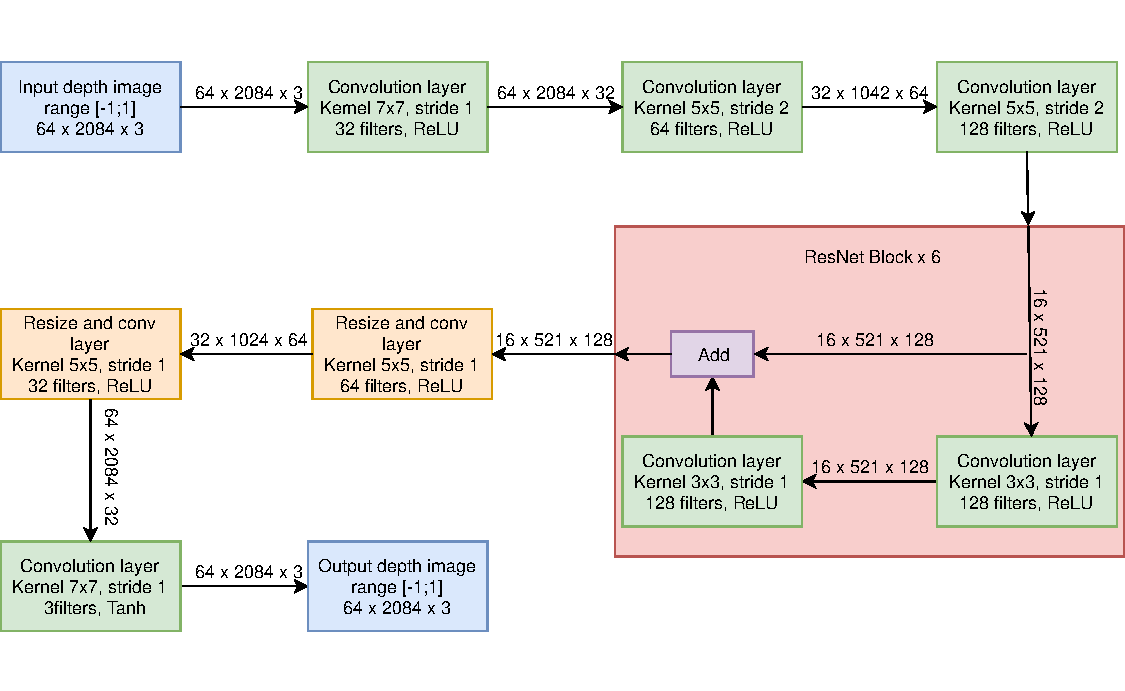
\includegraphics[keepaspectratio, width=0.98\textwidth]{img/gen.pdf}
\caption{Structure of the used generators}
\label{genstruct}
\end{figure}

The structure of the used discriminator can be seen at the figure \ref{disstruct}. Coloring is almost the same as in the figure \ref{genstruct}, however yellow node corresponds to the fully-connected layer.

\begin{figure}
\centering
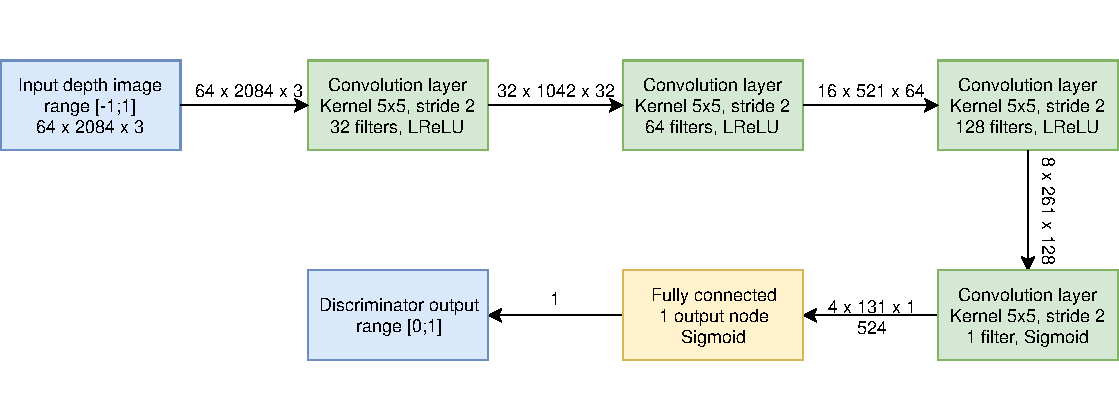
\includegraphics[keepaspectratio, width=0.98\textwidth]{img/disc.pdf}
\caption{Structure of the used discriminators}
\label{disstruct}
\end{figure}

The feature map for the self-regularization term of the generators' loss functions was formulated as follows -- if the pixel corresponding to the particular ray was valid (third channel) in both depth images (original and converted by the generator), then the feature corresponding to that pixel was its depth and intensity (i.e. identity on the first two channels), but if it was not valid in either of the depth images, then the feature map would return tuple (0, 0). The feature map had the shape of $64\times2084\times3$ as an input and $64\times2084\times2$ as its output shape.

All of the experiments used the history pool~\cite{historypool} with the size of the pool being 50. All of the trainable variables in the networks were initialized using the Xavier~\cite{xavier} initialization. The other important hyperparameters are: $\lambda_D = 1$, $\lambda_G = 1$, $\lambda_{cyc} = 3$, $\lambda_{GP} = 3$ (where applicable), $\lambda_{reg} = 3$ (where applicable).

\subsection{Results}

This subsection will show an example of the results generated by the trained generators in the CycleGAN model. Figure \ref{evalcmpg2v} shows data generated from the testing portion of the GTA dataset transformed into Valeo dataset by the means of different GANs used within CycleGAN model. Figure \ref{evalcmpg2vcutout} shows the same data, but only small part of the images is shown to ease the viewing. Note that while the part displayed in the depth and intensity images show the {\em same} part of the data, the portion displayed in the point cloud section does not correspond to the same part of the scene. The figures \ref{evalcmpv2g} and \ref{evalcmpv2gcutout} have the same layout, only they show the data transformed from the testing portion of the Valeo dataset to GTA dataset.

For more data see contents of the enclosed CD, as described in the appendix \ref{cd}

\begin{figure}
\begin{tabular}{L|III}
 & \textbf{Depth} & \textbf{Intensity} & \textbf{Point cloud} \\
Original & 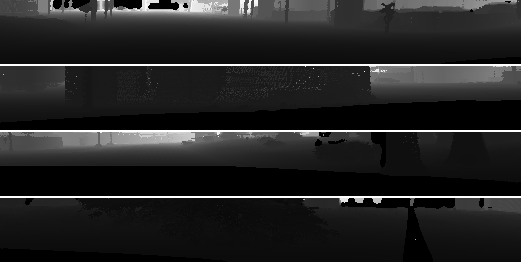
\includegraphics[keepaspectratio, width=0.98\linewidth]{img/gta2valeo-depthorig.png} & 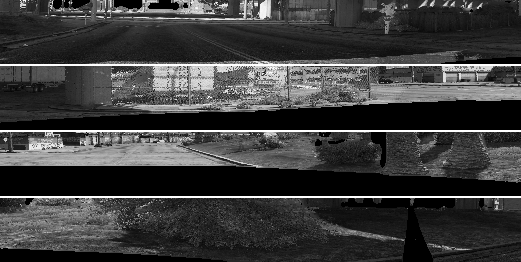
\includegraphics[keepaspectratio, width=0.98\linewidth]{img/gta2valeo-intenorig.png} & 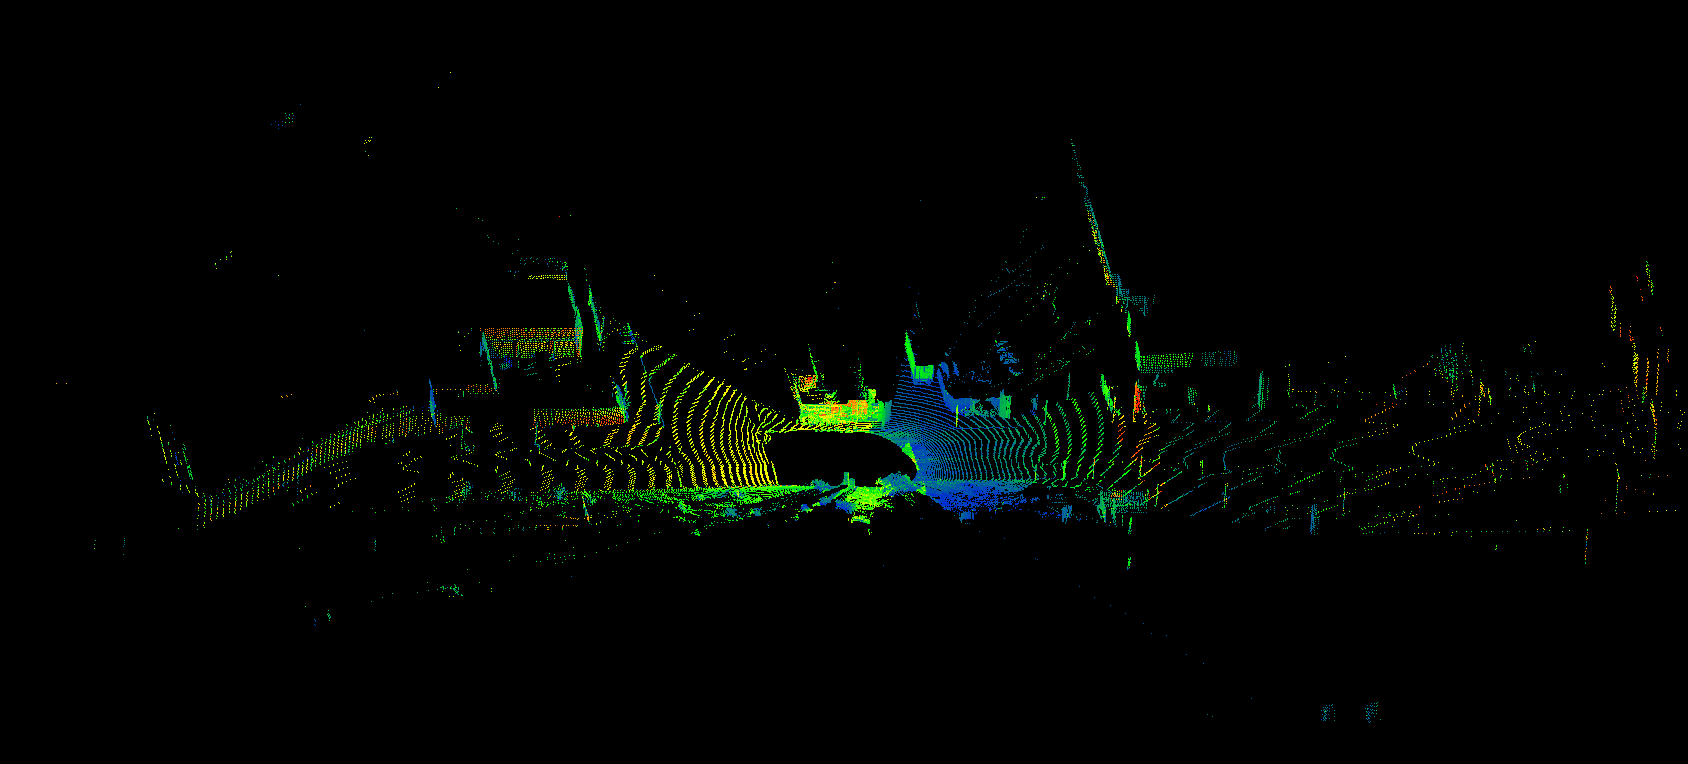
\includegraphics[keepaspectratio, width=0.98\linewidth]{img/gta2valeo-pclorig.png} \\
GAN\linebreak{}No Self-reg & 
\includegraphics[keepaspectratio, width=0.98\linewidth]{img/gta2valeo-depthgannosr.png} & 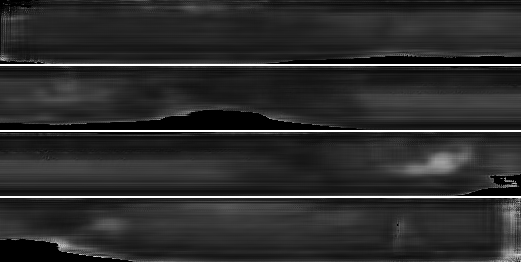
\includegraphics[keepaspectratio, width=0.98\linewidth]{img/gta2valeo-intengannosr.png} & 
\includegraphics[keepaspectratio, width=0.98\linewidth]{img/gta2valeo-pclgannosr.png} \\
GAN\linebreak{}Self-reg & 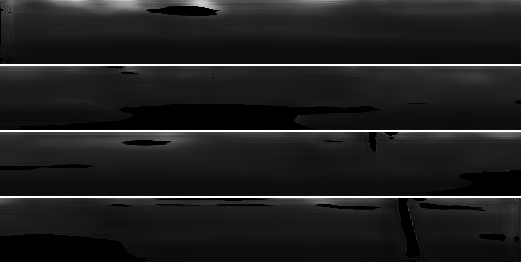
\includegraphics[keepaspectratio, width=0.98\linewidth]{img/gta2valeo-depthgansr.png} & 
\includegraphics[keepaspectratio, width=0.98\linewidth]{img/gta2valeo-intengansr.png} & 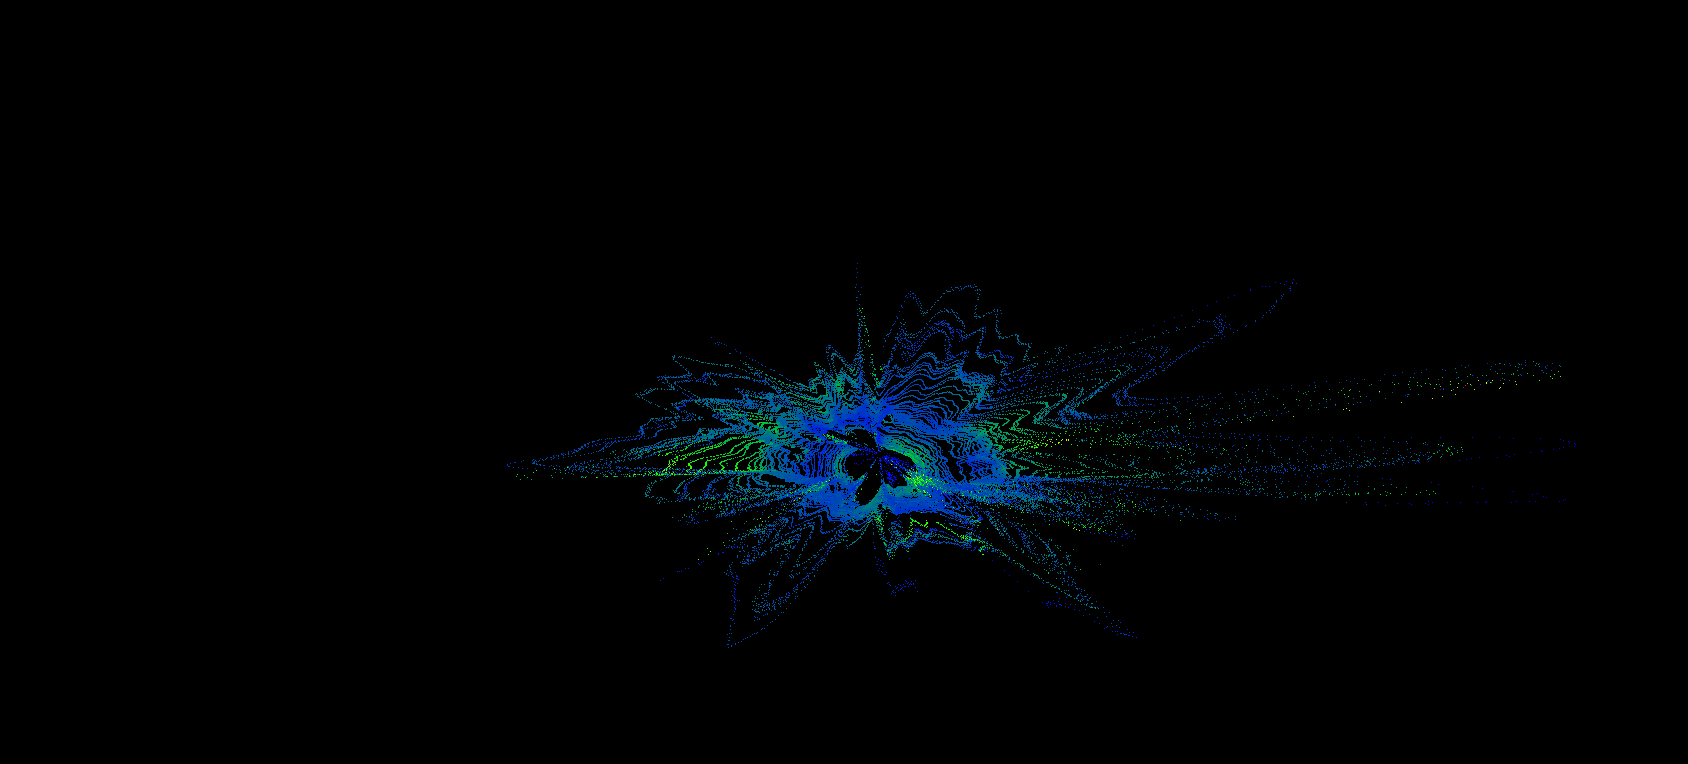
\includegraphics[keepaspectratio, width=0.98\linewidth]{img/gta2valeo-pclgansr.png} \\
LSGAN\linebreak{}No Self-reg & 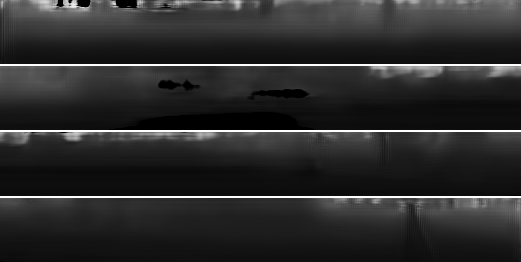
\includegraphics[keepaspectratio, width=0.98\linewidth]{img/gta2valeo-depthlsgannosr.png} & 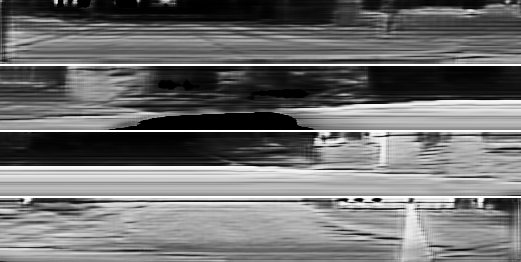
\includegraphics[keepaspectratio, width=0.98\linewidth]{img/gta2valeo-intenlsgannosr.png} & 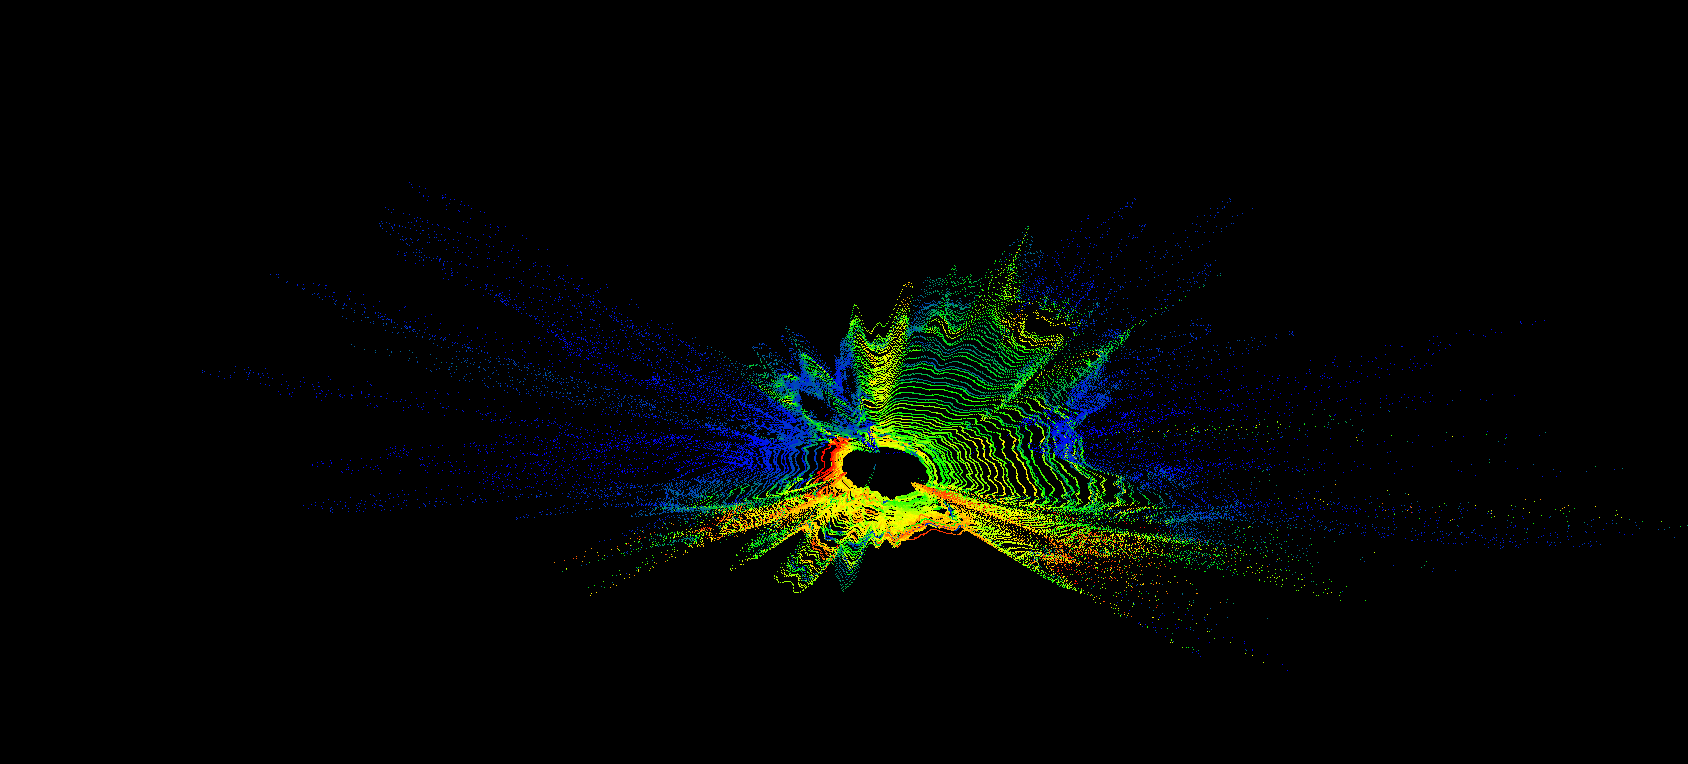
\includegraphics[keepaspectratio, width=0.98\linewidth]{img/gta2valeo-pcllsgannosr.png} \\
LSGAN\linebreak{}Self-reg & 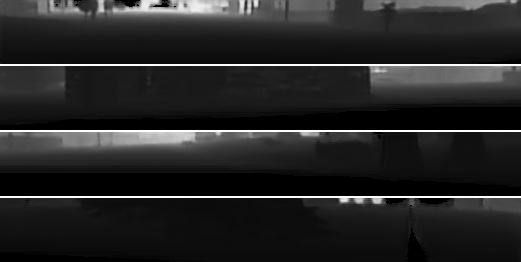
\includegraphics[keepaspectratio, width=0.98\linewidth]{img/gta2valeo-depthlsgansr.png} & 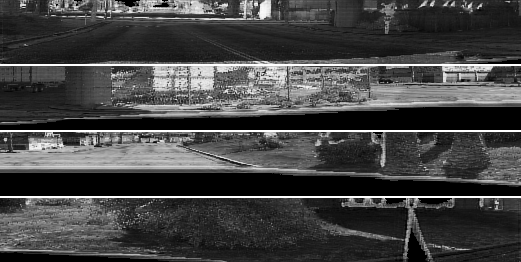
\includegraphics[keepaspectratio, width=0.98\linewidth]{img/gta2valeo-intenlsgansr.png} & 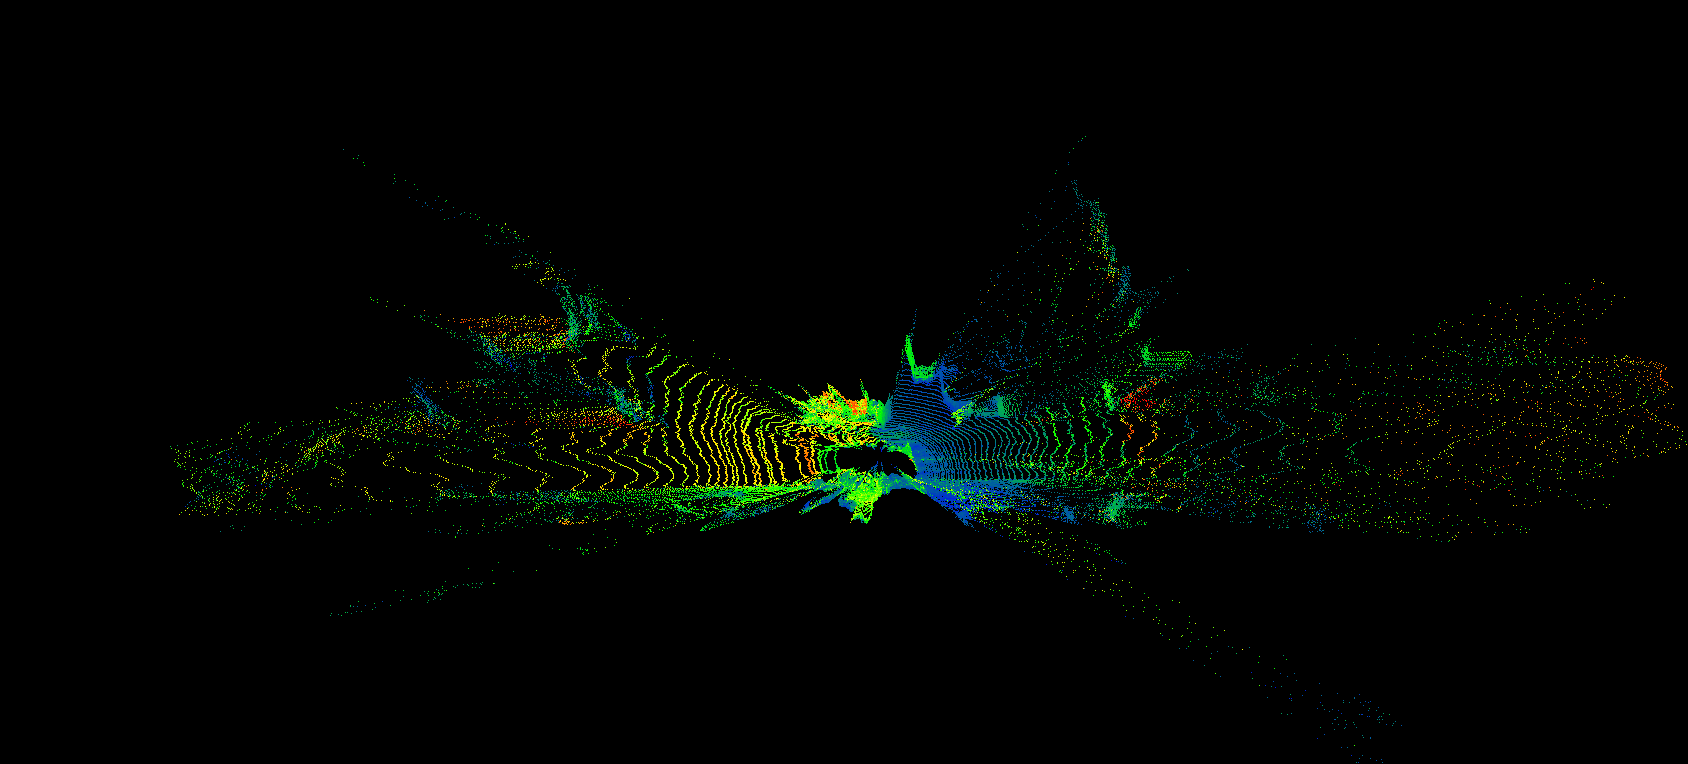
\includegraphics[keepaspectratio, width=0.98\linewidth]{img/gta2valeo-pcllsgansr.png} \\
WGAN-GP\linebreak{}No Self-reg & 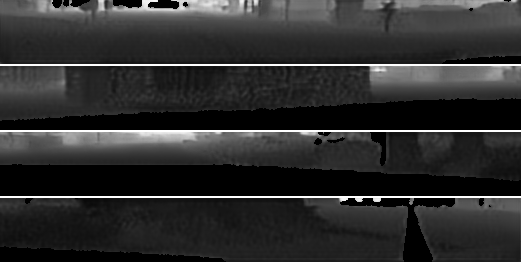
\includegraphics[keepaspectratio, width=0.98\linewidth]{img/gta2valeo-depthwgannosr.png} & 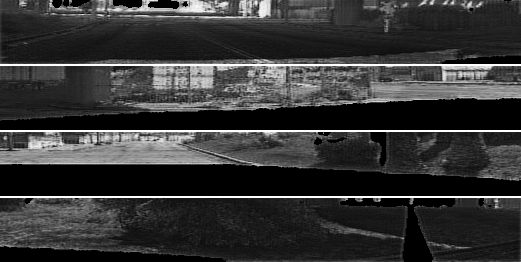
\includegraphics[keepaspectratio, width=0.98\linewidth]{img/gta2valeo-intenwgannosr.png} & 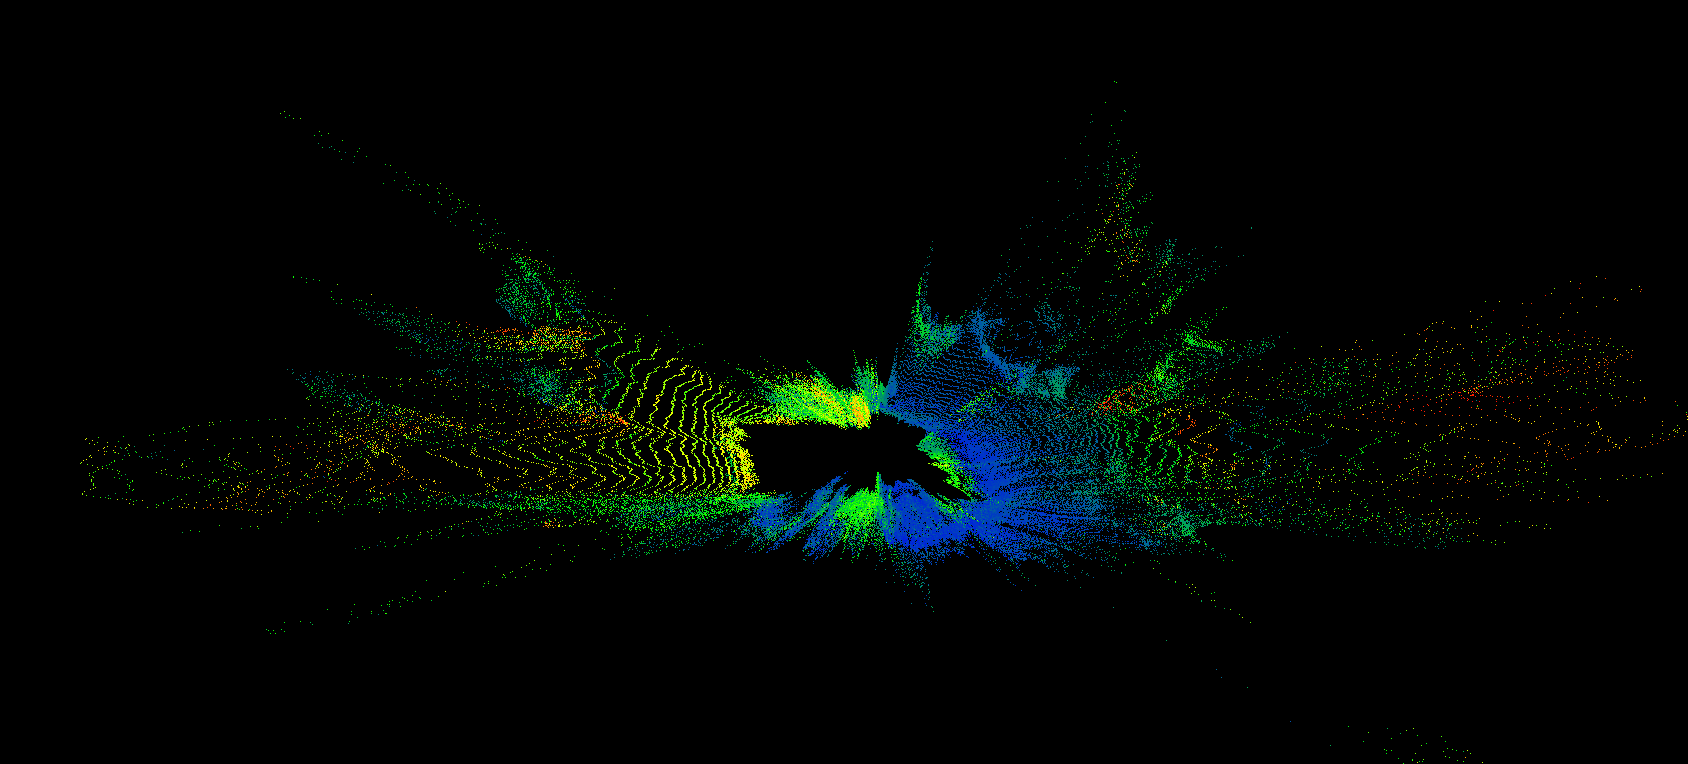
\includegraphics[keepaspectratio, width=0.98\linewidth]{img/gta2valeo-pclwgannosr.png} \\
WGAN-GP\linebreak{}Self-reg & 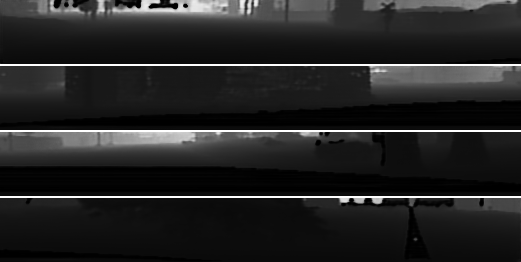
\includegraphics[keepaspectratio, width=0.98\linewidth]{img/gta2valeo-depthwgansr.png} & 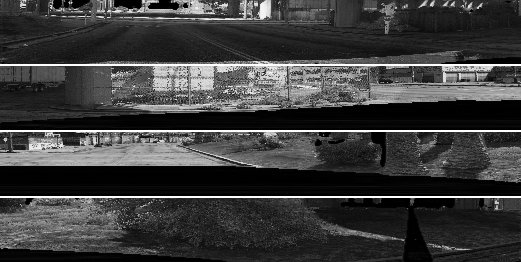
\includegraphics[keepaspectratio, width=0.98\linewidth]{img/gta2valeo-intenwgansr.png} & 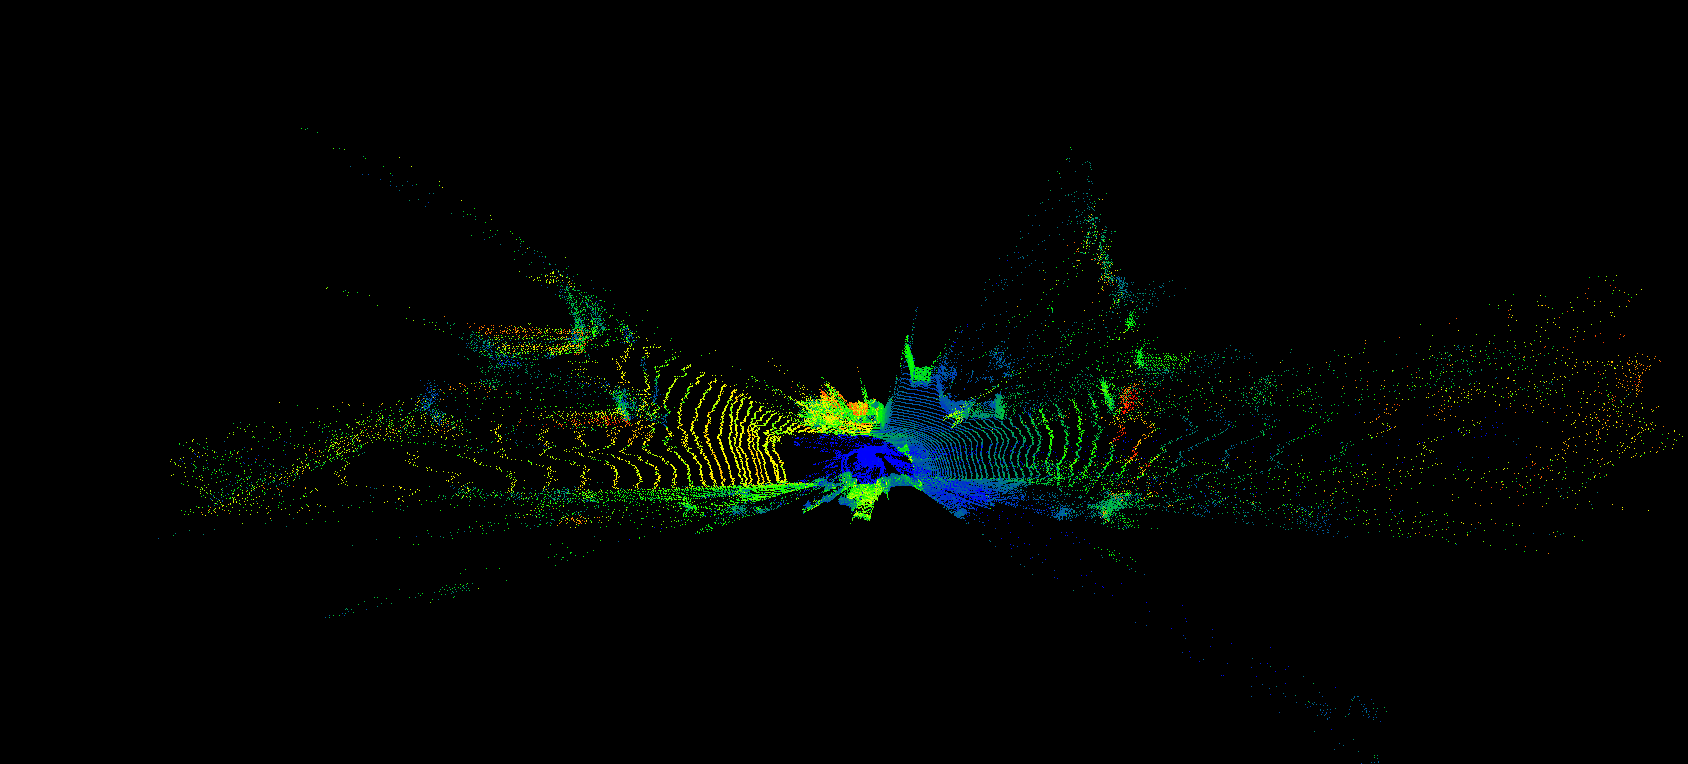
\includegraphics[keepaspectratio, width=0.98\linewidth]{img/gta2valeo-pclwgansr.png} \\
\end{tabular}
\centering
\caption{Comparison of different GAN variants used in CycleGAN, GTA to Valeo}
\label{evalcmpg2v}
\end{figure}

\begin{figure}
\begin{tabular}{L|III}
 & \textbf{Depth} & \textbf{Intensity} & \textbf{Point cloud} \\
Original & 
\includegraphics[keepaspectratio, width=0.98\linewidth]{img/gta2valeo-depthorigpart.png} & 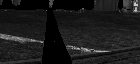
\includegraphics[keepaspectratio, width=0.98\linewidth]{img/gta2valeo-intenorigpart.png} & 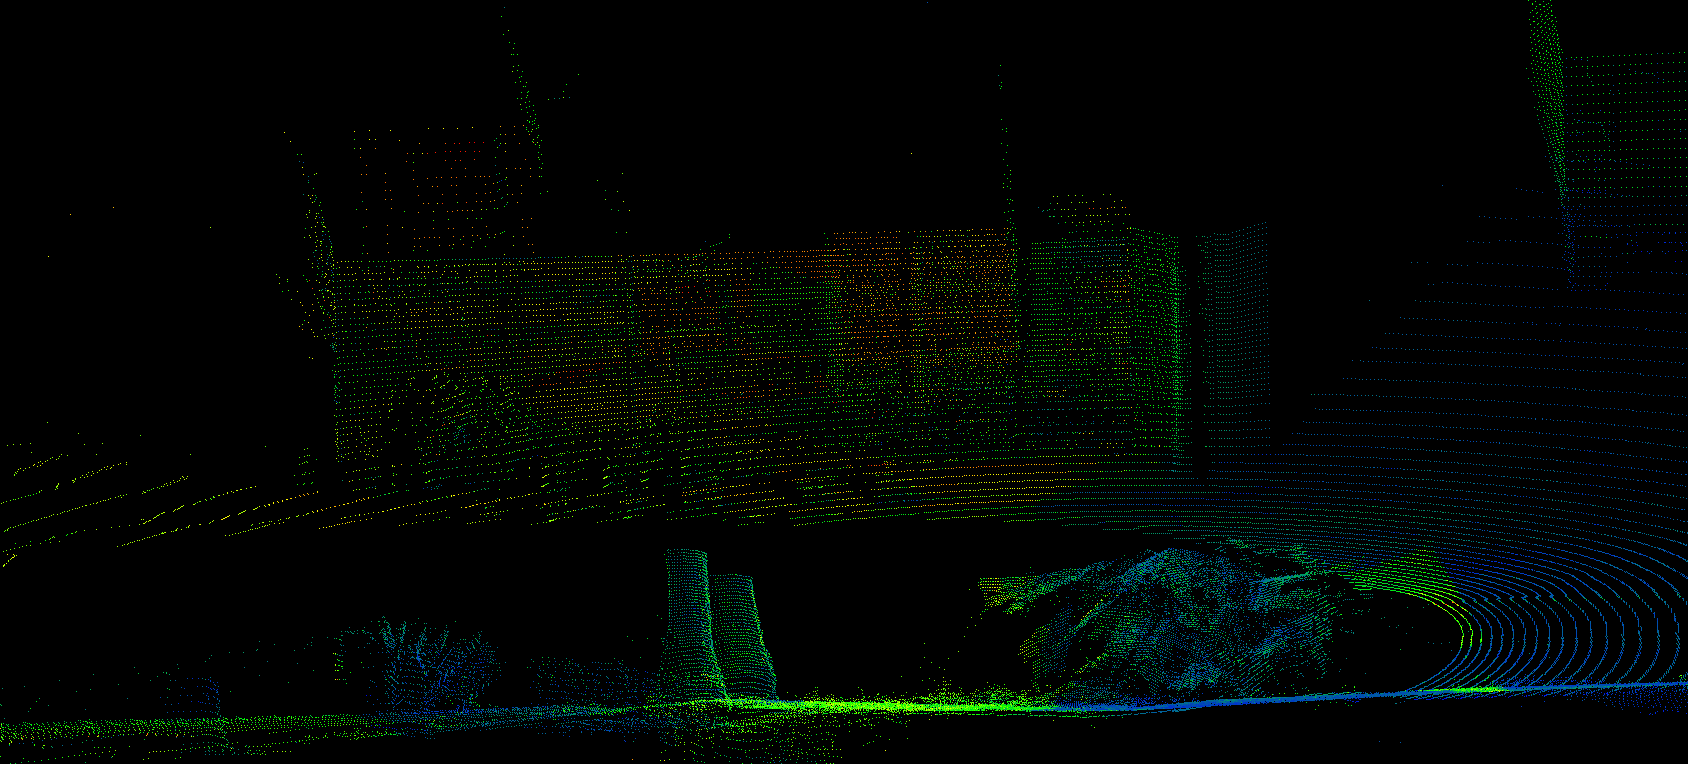
\includegraphics[keepaspectratio, width=0.98\linewidth]{img/gta2valeo-pclorigpart.png} \\
GAN\linebreak{}No Self-reg & 
\includegraphics[keepaspectratio, width=0.98\linewidth]{img/gta2valeo-depthgannosrpart.png} & 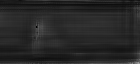
\includegraphics[keepaspectratio, width=0.98\linewidth]{img/gta2valeo-intengannosrpart.png} & 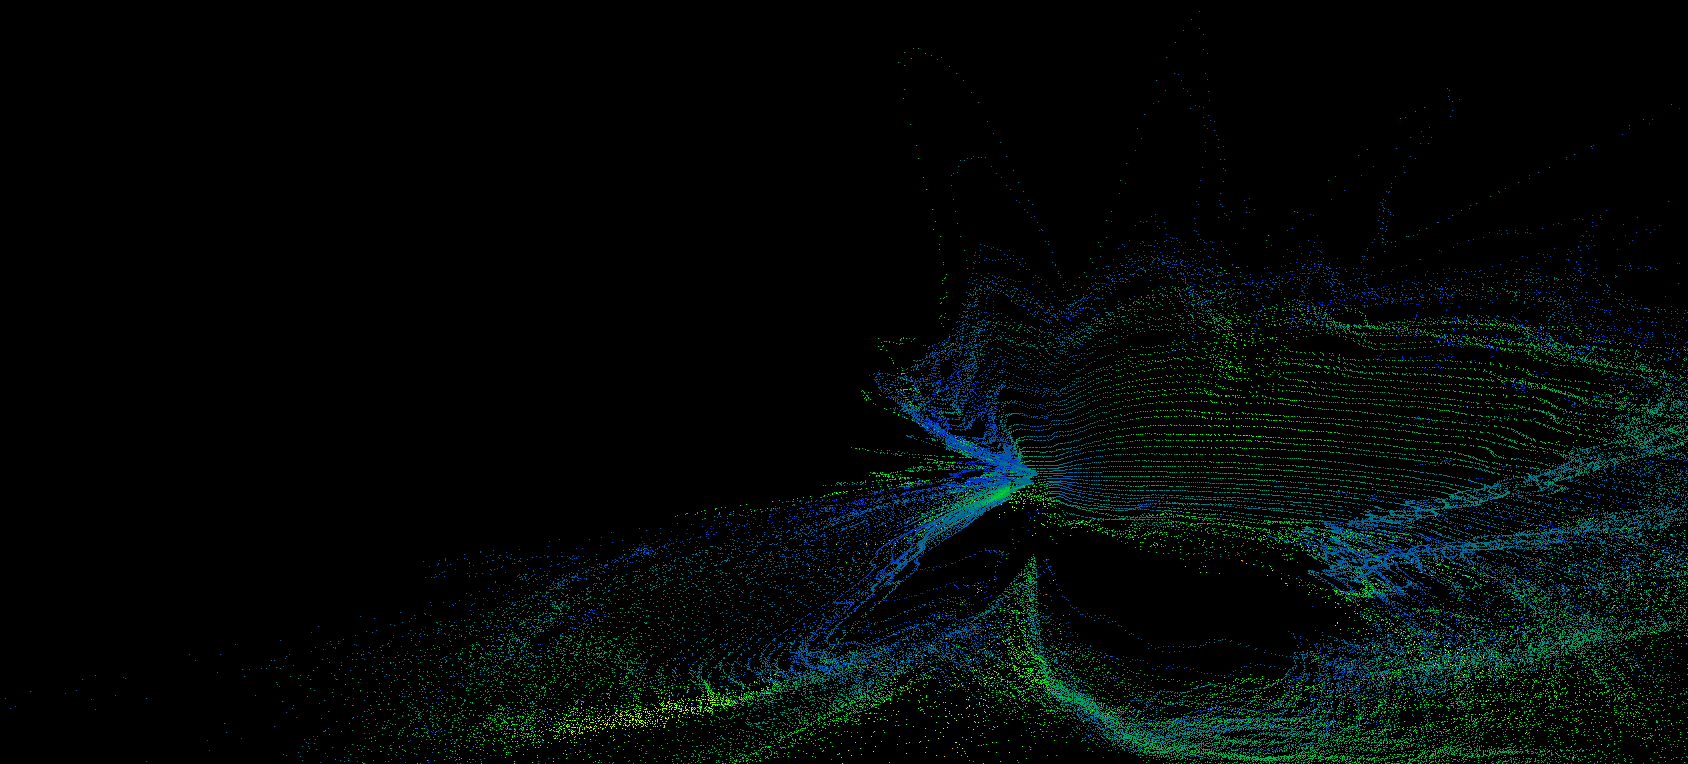
\includegraphics[keepaspectratio, width=0.98\linewidth]{img/gta2valeo-pclgannosrpart.png} \\
GAN\linebreak{}Self-reg & 
\includegraphics[keepaspectratio, width=0.98\linewidth]{img/gta2valeo-depthgansrpart.png} & 
\includegraphics[keepaspectratio, width=0.98\linewidth]{img/gta2valeo-intengansrpart.png} & 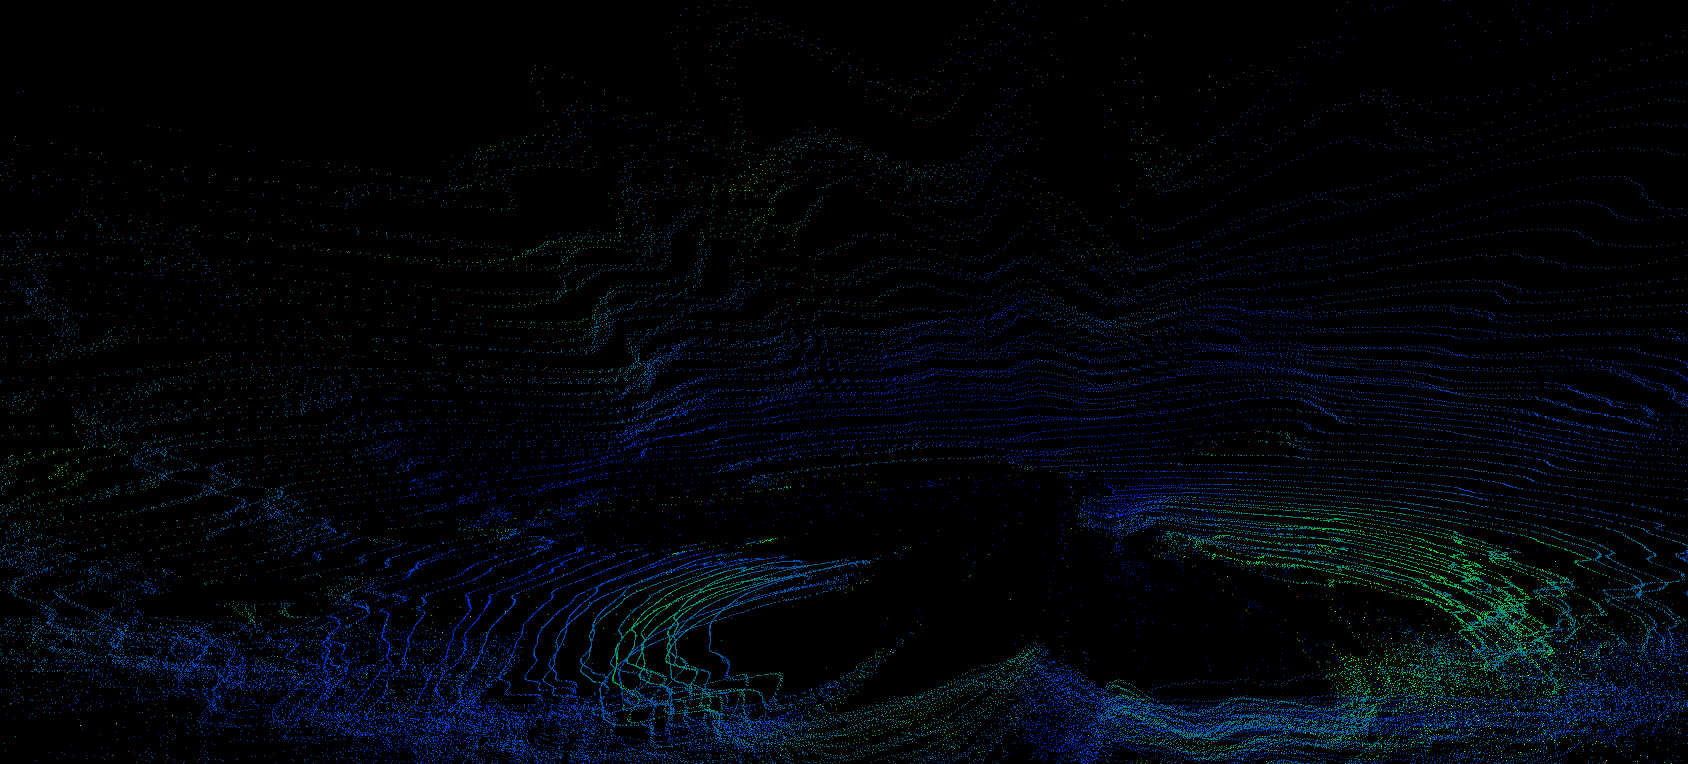
\includegraphics[keepaspectratio, width=0.98\linewidth]{img/gta2valeo-pclgansrpart.png} \\
LSGAN\linebreak{}No Self-reg & 
\includegraphics[keepaspectratio, width=0.98\linewidth]{img/gta2valeo-depthlsgannosrpart.png} & 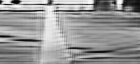
\includegraphics[keepaspectratio, width=0.98\linewidth]{img/gta2valeo-intenlsgannosrpart.png} & 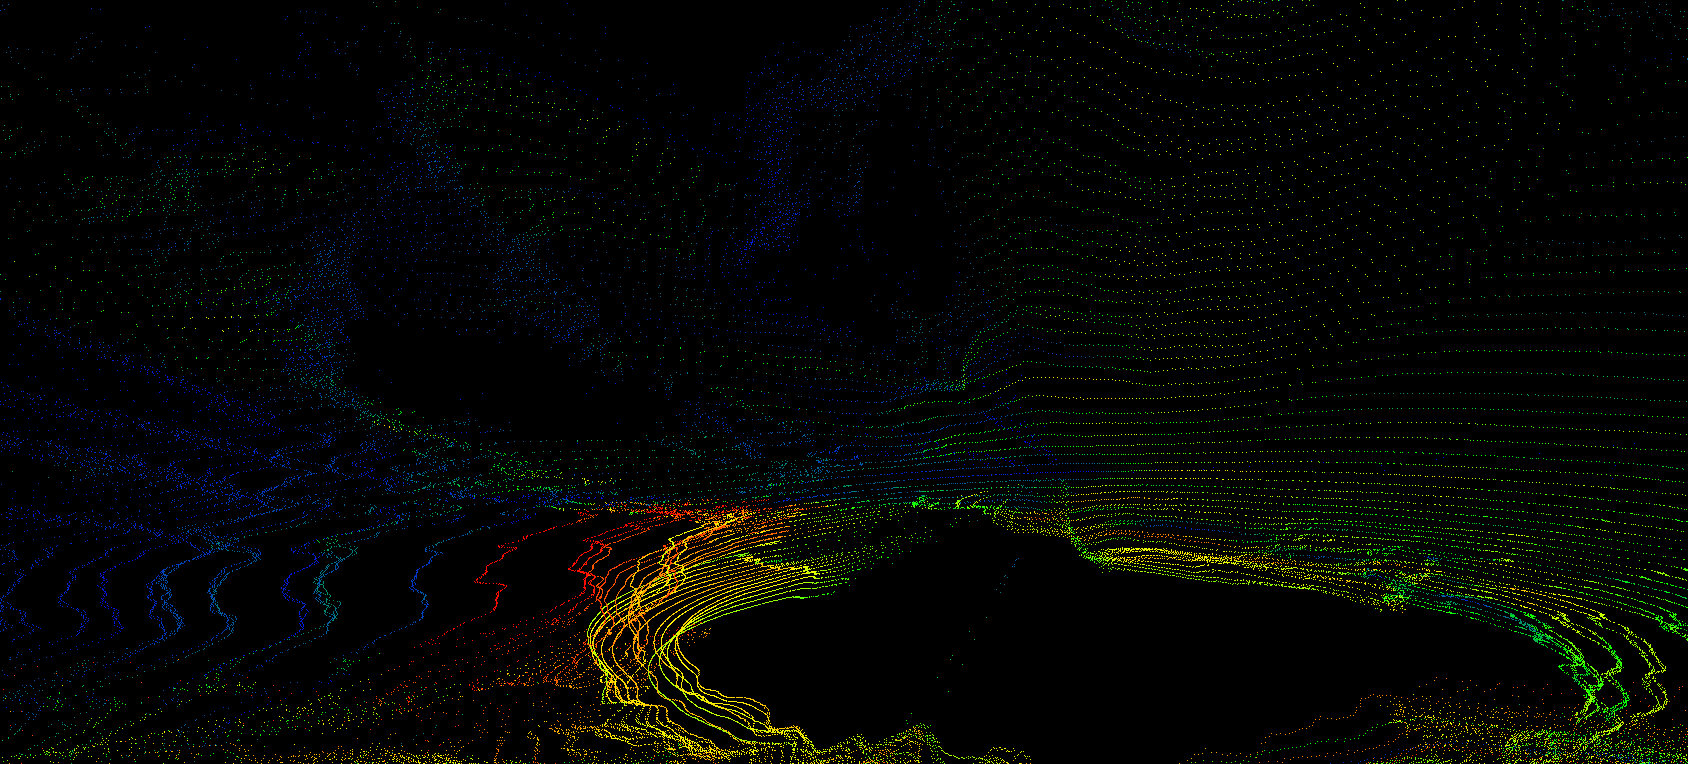
\includegraphics[keepaspectratio, width=0.98\linewidth]{img/gta2valeo-pcllsgannosrpart.png} \\
LSGAN\linebreak{}Self-reg & 
\includegraphics[keepaspectratio, width=0.98\linewidth]{img/gta2valeo-depthlsgansrpart.png} & 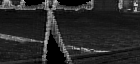
\includegraphics[keepaspectratio, width=0.98\linewidth]{img/gta2valeo-intenlsgansrpart.png} & 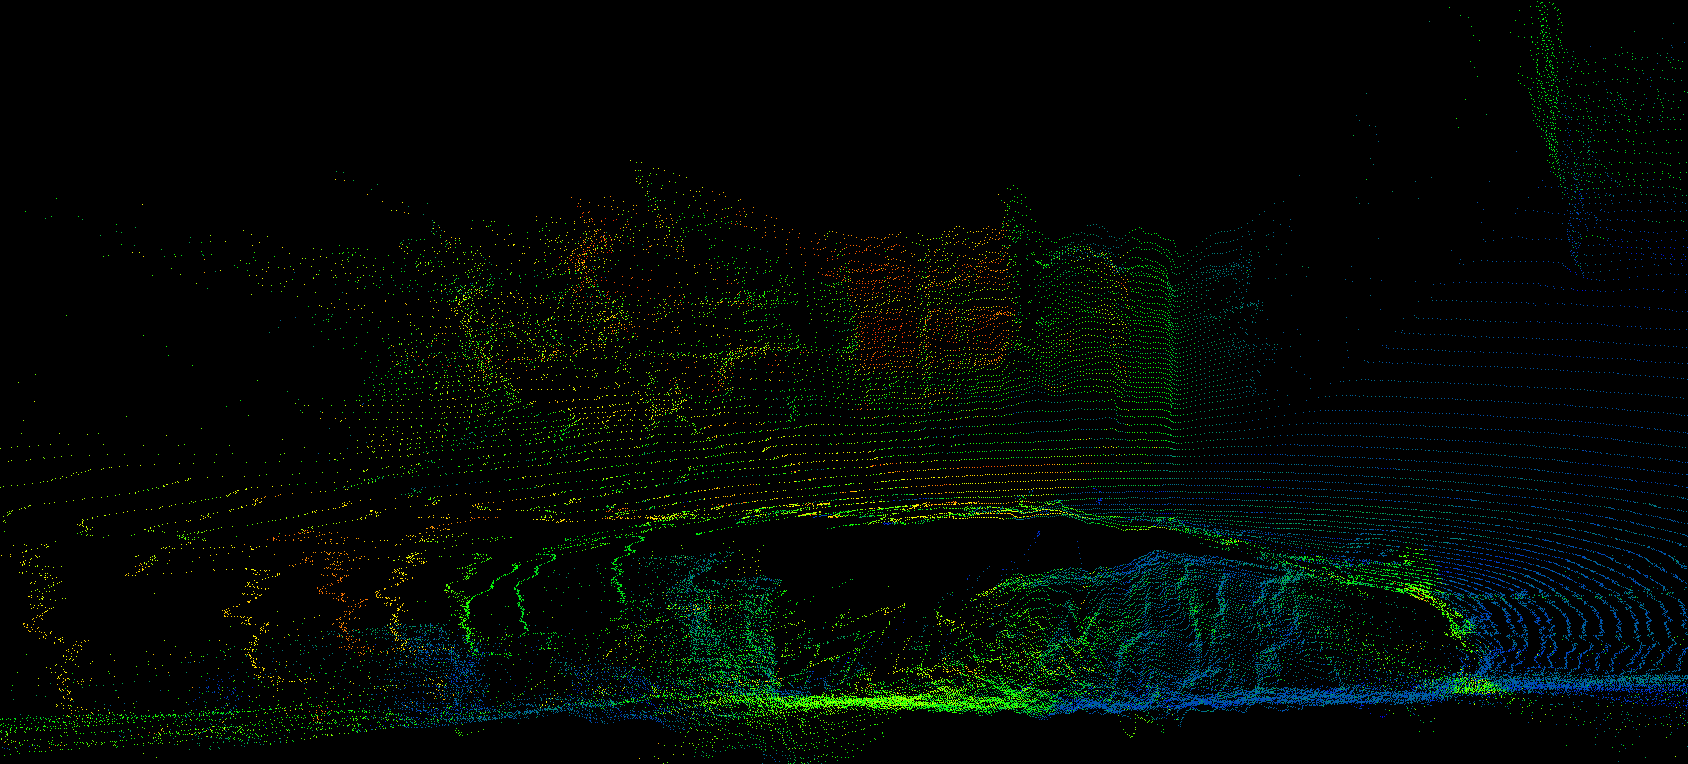
\includegraphics[keepaspectratio, width=0.98\linewidth]{img/gta2valeo-pcllsgansrpart.png} \\
WGAN-GP\linebreak{}No Self-reg & 
\includegraphics[keepaspectratio, width=0.98\linewidth]{img/gta2valeo-depthwgannosrpart.png} & 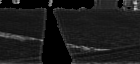
\includegraphics[keepaspectratio, width=0.98\linewidth]{img/gta2valeo-intenwgannosrpart.png} & 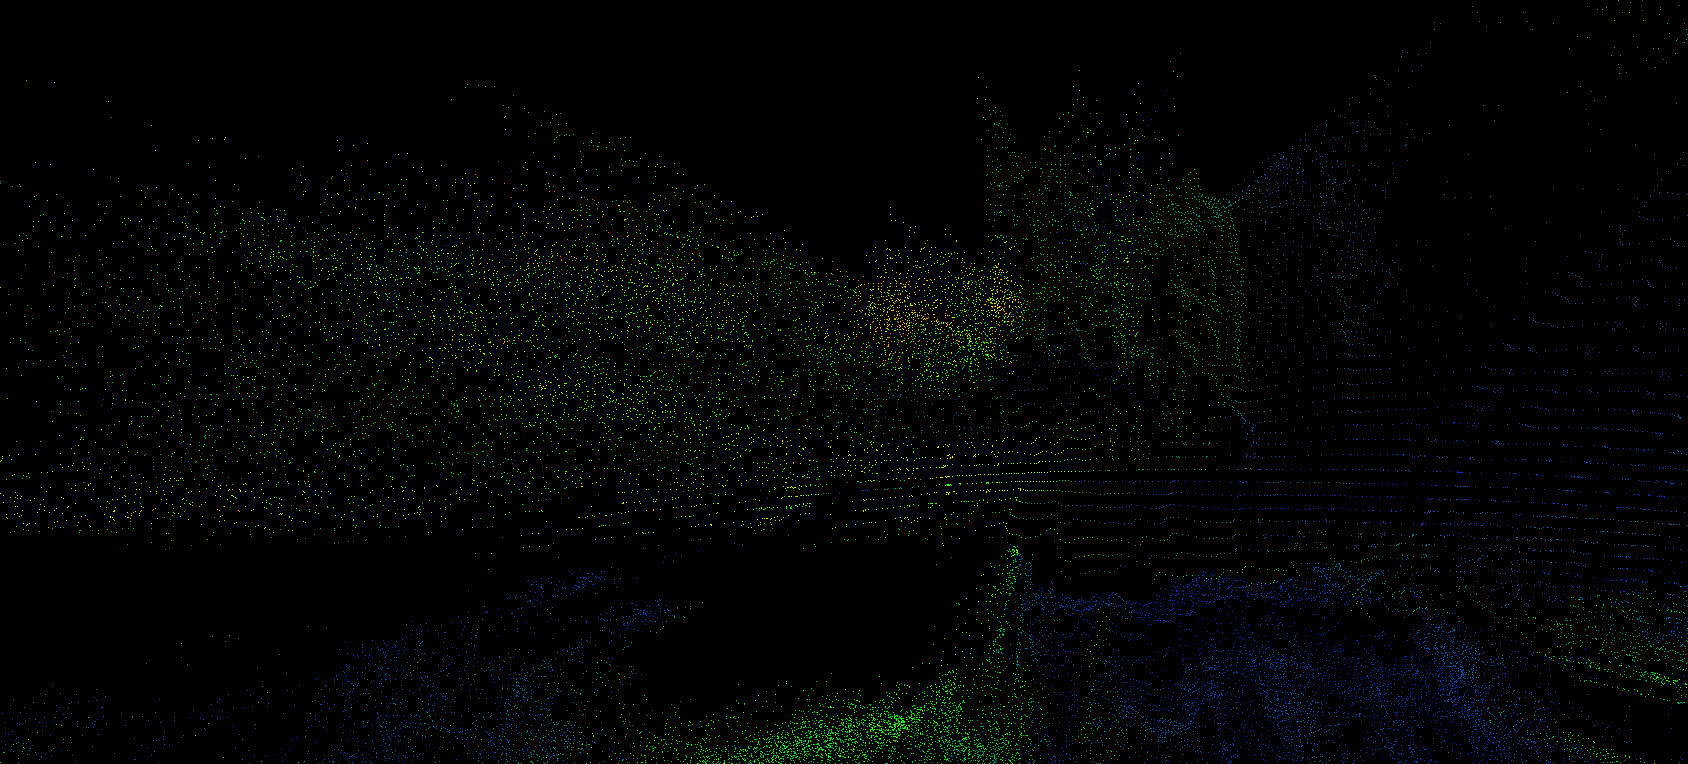
\includegraphics[keepaspectratio, width=0.98\linewidth]{img/gta2valeo-pclwgannosrpart.png} \\
WGAN-GP\linebreak{}Self-reg & 
\includegraphics[keepaspectratio, width=0.98\linewidth]{img/gta2valeo-depthwgansrpart.png} & 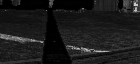
\includegraphics[keepaspectratio, width=0.98\linewidth]{img/gta2valeo-intenwgansrpart.png} & 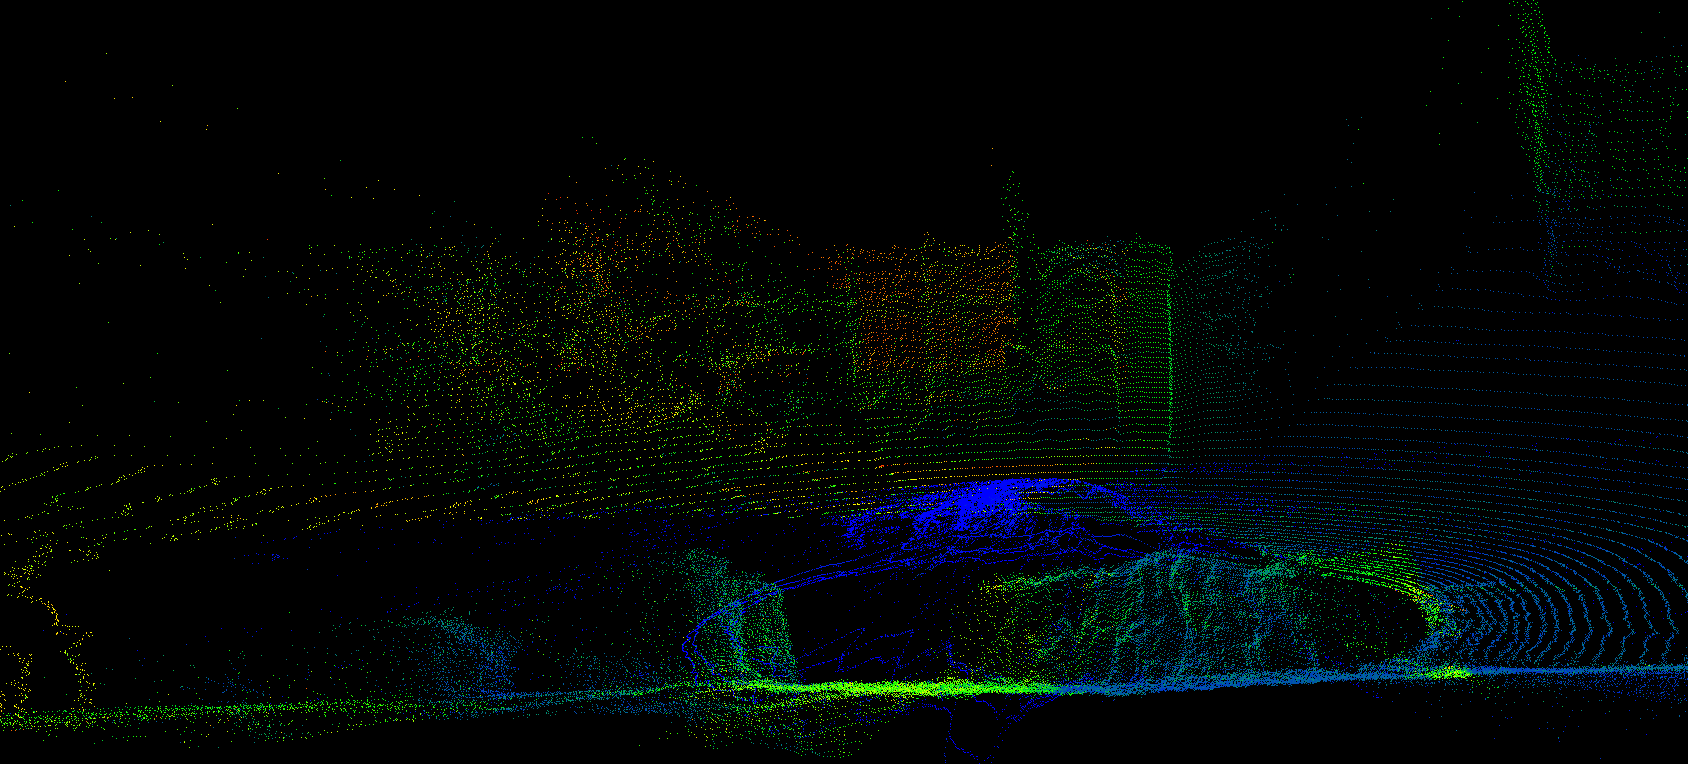
\includegraphics[keepaspectratio, width=0.98\linewidth]{img/gta2valeo-pclwgansrpart.png} \\
\end{tabular}
\centering
\caption[Comparison of different GAN variants used in CycleGAN, GTA to Valeo, cutout]{Comparison of different GAN variants used in CycleGAN, in a GTA to Valeo direction. Only a small part of the image is shown for better clarity.}
\label{evalcmpg2vcutout}
\end{figure}

\begin{figure}
\begin{tabular}{L|III}
 & \textbf{Depth} & \textbf{Intensity} & \textbf{Point cloud} \\
Original & 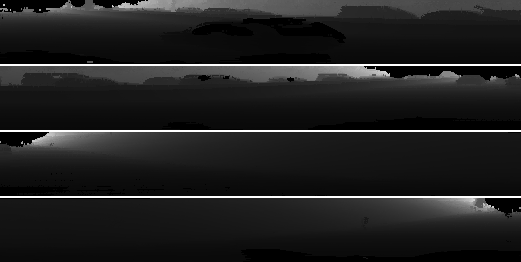
\includegraphics[keepaspectratio, width=0.98\linewidth]{img/valeo2gta-depthorig.png} & 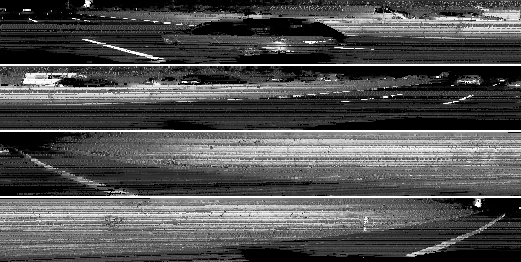
\includegraphics[keepaspectratio, width=0.98\linewidth]{img/valeo2gta-intenorig.png} & 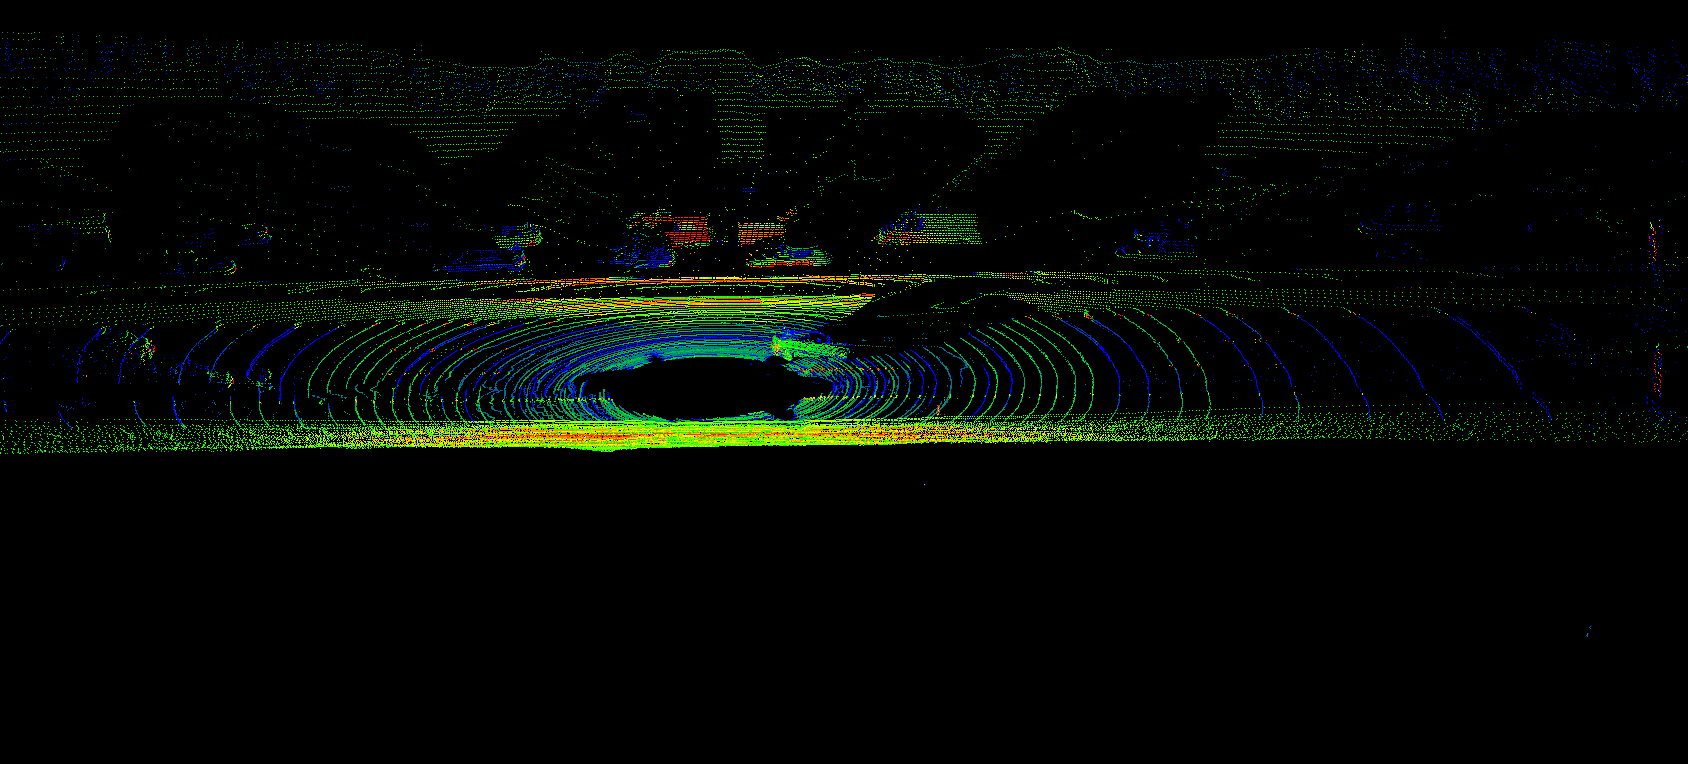
\includegraphics[keepaspectratio, width=0.98\linewidth]{img/valeo2gta-pclorig.png} \\
GAN\linebreak{}No Self-reg & 
\includegraphics[keepaspectratio, width=0.98\linewidth]{img/valeo2gta-depthgannosr.png} & 
\includegraphics[keepaspectratio, width=0.98\linewidth]{img/valeo2gta-intengannosr.png} & 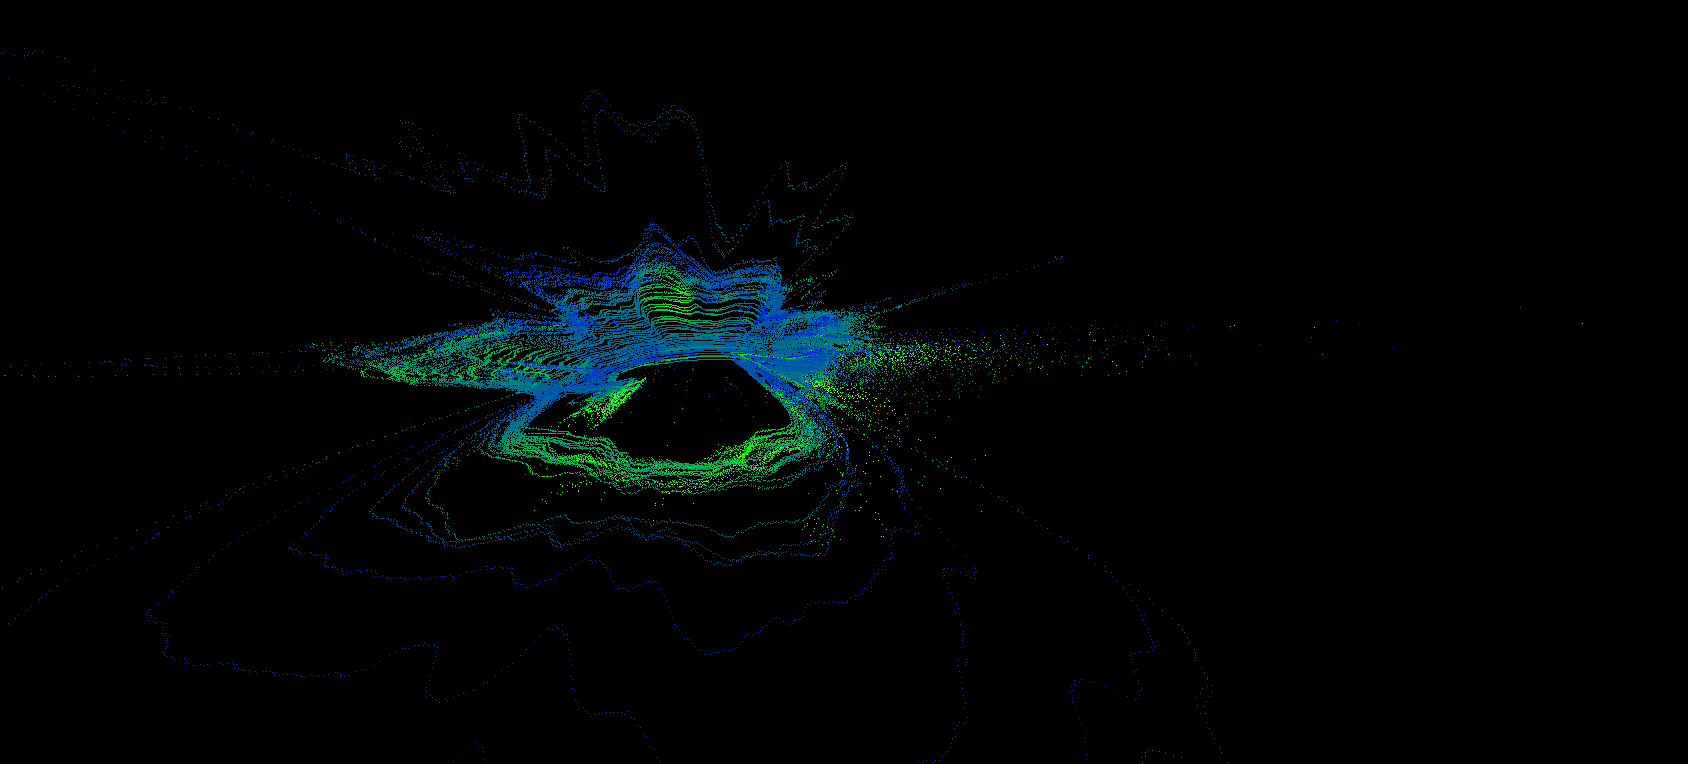
\includegraphics[keepaspectratio, width=0.98\linewidth]{img/valeo2gta-pclgannosr.png} \\
GAN\linebreak{}Self-reg & \includegraphics[keepaspectratio, width=0.98\linewidth]{img/valeo2gta-depthgansr.png} & \includegraphics[keepaspectratio, width=0.98\linewidth]{img/valeo2gta-intengansr.png} & \includegraphics[keepaspectratio, width=0.98\linewidth]{img/valeo2gta-pclgansr.png} \\
LSGAN\linebreak{}No Self-reg & \includegraphics[keepaspectratio, width=0.98\linewidth]{img/valeo2gta-depthlsgannosr.png} & \includegraphics[keepaspectratio, width=0.98\linewidth]{img/valeo2gta-intenlsgannosr.png} & \includegraphics[keepaspectratio, width=0.98\linewidth]{img/valeo2gta-pcllsgannosr.png} \\
LSGAN\linebreak{}Self-reg & \includegraphics[keepaspectratio, width=0.98\linewidth]{img/valeo2gta-depthlsgansr.png} & \includegraphics[keepaspectratio, width=0.98\linewidth]{img/valeo2gta-intenlsgansr.png} & \includegraphics[keepaspectratio, width=0.98\linewidth]{img/valeo2gta-pcllsgansr.png} \\
WGAN-GP\linebreak{}No Self-reg & \includegraphics[keepaspectratio, width=0.98\linewidth]{img/valeo2gta-depthwgannosr.png} & \includegraphics[keepaspectratio, width=0.98\linewidth]{img/valeo2gta-intenwgannosr.png} & \includegraphics[keepaspectratio, width=0.98\linewidth]{img/valeo2gta-pclwgannosr.png} \\
WGAN-GP\linebreak{}Self-reg & \includegraphics[keepaspectratio, width=0.98\linewidth]{img/valeo2gta-depthwgansr.png} & \includegraphics[keepaspectratio, width=0.98\linewidth]{img/valeo2gta-intenwgansr.png} & \includegraphics[keepaspectratio, width=0.98\linewidth]{img/valeo2gta-pclwgansr.png} \\
\end{tabular}
\centering
\caption{Comparison of different GAN variants used in CycleGAN, Valeo to GTA}
\label{evalcmpv2g}
\end{figure}

\begin{figure}
\begin{tabular}{L|III}
 & \textbf{Depth} & \textbf{Intensity} & \textbf{Point cloud} \\
Original & \includegraphics[keepaspectratio, width=0.98\linewidth]{img/valeo2gta-depthorigpart.png} & \includegraphics[keepaspectratio, width=0.98\linewidth]{img/valeo2gta-intenorigpart.png} & \includegraphics[keepaspectratio, width=0.98\linewidth]{img/valeo2gta-pclorigpart.png} \\
GAN\linebreak{}No Self-reg & \includegraphics[keepaspectratio, width=0.98\linewidth]{img/valeo2gta-depthgannosrpart.png} & \includegraphics[keepaspectratio, width=0.98\linewidth]{img/valeo2gta-intengannosrpart.png} & \includegraphics[keepaspectratio, width=0.98\linewidth]{img/valeo2gta-pclgannosrpart.png} \\
GAN\linebreak{}Self-reg & \includegraphics[keepaspectratio, width=0.98\linewidth]{img/valeo2gta-depthgansrpart.png} & \includegraphics[keepaspectratio, width=0.98\linewidth]{img/valeo2gta-intengansrpart.png} & \includegraphics[keepaspectratio, width=0.98\linewidth]{img/valeo2gta-pclgansrpart.png} \\
LSGAN\linebreak{}No Self-reg & \includegraphics[keepaspectratio, width=0.98\linewidth]{img/valeo2gta-depthlsgannosrpart.png} & \includegraphics[keepaspectratio, width=0.98\linewidth]{img/valeo2gta-intenlsgannosrpart.png} & \includegraphics[keepaspectratio, width=0.98\linewidth]{img/valeo2gta-pcllsgannosrpart.png} \\
LSGAN\linebreak{}Self-reg & \includegraphics[keepaspectratio, width=0.98\linewidth]{img/valeo2gta-depthlsgansrpart.png} & \includegraphics[keepaspectratio, width=0.98\linewidth]{img/valeo2gta-intenlsgansrpart.png} & \includegraphics[keepaspectratio, width=0.98\linewidth]{img/valeo2gta-pcllsgansrpart.png} \\
WGAN-GP\linebreak{}No Self-reg & \includegraphics[keepaspectratio, width=0.98\linewidth]{img/valeo2gta-depthwgannosrpart.png} & \includegraphics[keepaspectratio, width=0.98\linewidth]{img/valeo2gta-intenwgannosrpart.png} & \includegraphics[keepaspectratio, width=0.98\linewidth]{img/valeo2gta-pclwgannosrpart.png} \\
WGAN-GP\linebreak{}Self-reg & \includegraphics[keepaspectratio, width=0.98\linewidth]{img/valeo2gta-depthwgansrpart.png} & \includegraphics[keepaspectratio, width=0.98\linewidth]{img/valeo2gta-intenwgansrpart.png} & \includegraphics[keepaspectratio, width=0.98\linewidth]{img/valeo2gta-pclwgansrpart.png} \\
\end{tabular}
\centering
\caption[Comparison of different GAN variants used in CycleGAN, Valeo to GTA, cutout]{Comparison of different GAN variants used in CycleGAN, in a Valeo to GTA direction. Only a small part of the image is shown for better clarity.}
\label{evalcmpv2gcutout}
\end{figure}
